\section{Instruction Management Unit (Unité de gestion des instructions)}

\subsection{Design Instruction Management Unit}

The 32-bit instruction management unit possesses some properties:
\begin{itemize}
    \item An instruction memory of 64 words of 32 bits similar to that 
    of the processing unit.
    \item There is no write data bus and Write Enable.
    \item A 32-bit register (PC register) which has a clock and a
    asynchronous reset (active at high level).
    \item An extension unit of 24 to 32 signed bits similar to the component \texttt{Extension} described
    previously.
\end{itemize}

A symbolic representation of an Instruction Management Unit
is shown in Figure \ref{fig:IMU}.

\begin{figure}[htp]
    \centering
    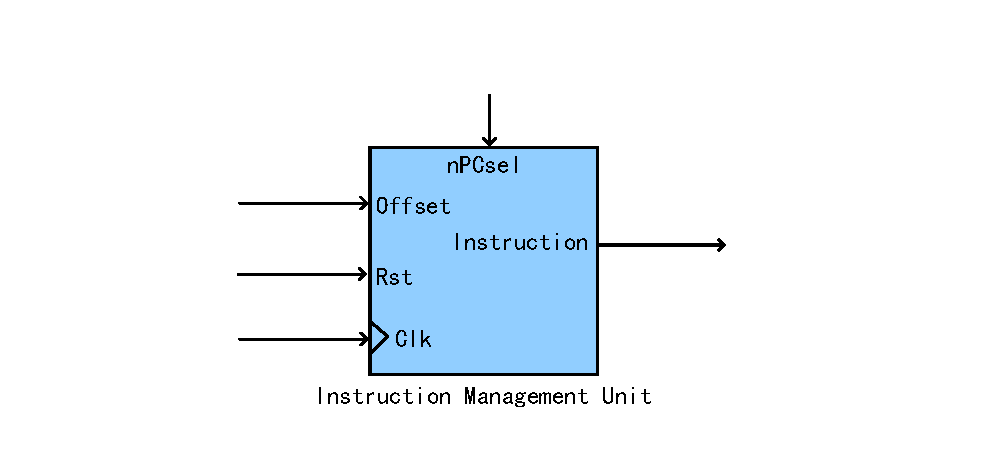
\includegraphics[width=0.5\textwidth]{picture/IMU.pdf}
    \caption{Instruction Management Unit Block Diagram}     
    \label{fig:IMU}
\end{figure}

Abstracted by the given block diagram, 
the function of the instruction management unit can be 
discribed as follow:
\begin{equation*}
    \texttt{PC} = \begin{cases}
        \texttt{PC} + 1 & \texttt{nPCsel} = 0 \\
        \texttt{PC} + 1 + \texttt{offset} & \texttt{nPCsel} = 1
    \end{cases}
\end{equation*} 

Because the instructions given are 24-bit, we need to use component \texttt{Extension} to extend them to 32-bit.
After that, we store these 32-bit instructions in memory by \texttt{Datamemory}.

The part of the source in \textbf{Instruction\_Management\_Unit.vhd} will be given below.
\begin{lstlisting}[style=vhdl,breaklines]
architecture behave of Instruction_Management_Unit is
	signal PC, S : std_logic_vector(31 downto 0);  
begin

	Instruction_memory : entity work.instruction_memory port map (PC=> PC, Instruction=> Instruction); 
	Sign_Extension  : entity work.Sign_Extension  generic map(N=> 24) port map ( E => Offset, S => S); 

	process(clk, rst) 
	begin 
        if rst ='1' then 
            PC <= (others => '0'); 
        elsif rising_edge(clk) then 
            if nPCsel = '0' then 
                PC <= std_logic_vector(unsigned(PC)+1);	
            else 
                PC <= std_logic_vector(unsigned(PC)+1+ unsigned(S));	
            end if; 
        end if; 
	end process; 
end architecture;
\end{lstlisting}

And here is the code \textbf{instruction\_memory.vhd} in Appendices \ref{AppendicesA}.

\begin{lstlisting}[style=vhdl, columns=fixed,breaklines]
library IEEE;
use IEEE.std_logic_1164.all;
use IEEE.numeric_std.all;

entity instruction_memory is
    port(
        PC: in std_logic_vector(31 downto 0);
        Instruction: out std_logic_vector(31 downto 0)
    );
end entity;

architecture RTL of instruction_memory is
    type RAM64x32 is array(0 to 63) of std_logic_vector(31 downto 0);
    
function init_mem return RAM64x32 is 
    variable result : RAM64x32;
begin
    for i in 63 downto 0 loop
        result(i) := (others => '0');
    end loop;					 -- PC        -- INSTRUCTION  
        result(0) := x"E3A01020";-- 0x0 _main -- MOV R1,#0x20 
        result(1) := x"E3A02000";-- 0x1		  -- MOV R2,#0x00 
        result(2) := x"E6110000";-- 0x2 _loop -- LDR R0,0(R1)  
        result(3) := x"E0822000";-- 0x3		  -- ADD R2,R2,R0 
        result(4) := x"E2811001";-- 0x4		  -- ADD R1,R1,#1 
        result(5) := x"E351002A";-- 0x5		  -- CMP R1,0x2A  
        result(6) := x"BAFFFFFB";-- 0x6		  -- BLT loop 	 
        result(7) := x"E6012000";-- 0x7		  -- STR R2,0(R1) 
        result(8) := x"EAFFFFF7";-- 0x8		  -- BAL main	 
    return result;
end init_mem;	

signal mem: RAM64x32 := init_mem;

begin 
    Instruction <= mem(to_integer(unsigned(PC)));
end architecture;
	
\end{lstlisting}

\subsection{Simulation for Instruction Management Unit}
\label{sec:Simulation for Instruction Management Unit}

We build the testbench in order to test whether this unit work properly.


We mainly test the instruction such as
\begin{center}
        \texttt{PC} <= \texttt{PC} + 1 \\
        \texttt{PC} <=\texttt{PC} + 1 + \texttt{offset}
\end{center}
and change the value of \texttt{offset}$=\{1,-1\}$.

Given the code of the testbench \textbf{Instruction\_Management\_Unit\_tb.vhd} as follow.
\begin{lstlisting}[style=vhdl,columns=fixed, breaklines]
library ieee;
use ieee.std_logic_1164.all;
use ieee.numeric_std.all;

entity Instruction_Management_Unit_tb IS  
end entity ;
    
architecture BENCH of Instruction_Management_Unit_tb is
    signal Instruction : std_logic_vector(31 downto 0);
    signal Clk         : std_logic := '0';
    signal rst, nPCsel : std_logic;
    signal Offset      : std_logic_vector(23 downto 0);
    signal Done        : boolean := False; 
    constant Period    : time := 20 ns;
begin
    
    UUT : entity work.Instruction_Management_Unit port map(clk=>clk, rst=> rst, nPCsel =>nPCsel, Offset => Offset,Instruction => Instruction); 
    
    CLK <= '0' when Done else not CLK after Period / 2;
    Rst <= '1', '0' after 5 ns; 
    
    process
    begin
        
        nPCsel<= '0'; 
        Offset <= (others => '0'); -- PC <= PC + 1 
        wait for 20 ns;
        
        nPCsel<= '0'; 
        Offset <= (others => '0'); -- PC <= PC + 1 
        wait for 20 ns;
        
        nPCsel<= '1'; 
        Offset <= x"000001"; -- PC <= PC + 1 + Offset 1 
        wait for 20 ns;
        
        nPCsel<= '0'; 
        Offset <= (others => '0'); -- PC <= PC + 1
        wait for 20 ns;
        
        nPCsel<= '1'; 
        Offset <= x"FFFFFF"; -- PC <= PC + 1 + Offset -1 
        wait for 20 ns;
        
        nPCsel<= '0'; 
        Offset <= (others => '0'); -- PC <= PC + 1 
        wait for 20 ns;
        
        Done <= True; 
        wait;
        
    end process;
    
end architecture;    
\end{lstlisting}

With the command file \textbf{Instruction\_Management\_Unit\_test.do}, the waves of the simulation are shown as Figure \ref{fig:IMUres}. Detailed waves can be found as Figure \ref{fig:ModelSim_ insmanagement_tb(bench)} in Appendices \ref{AppendicesA}.

\begin{figure}[htp]
    \centering
    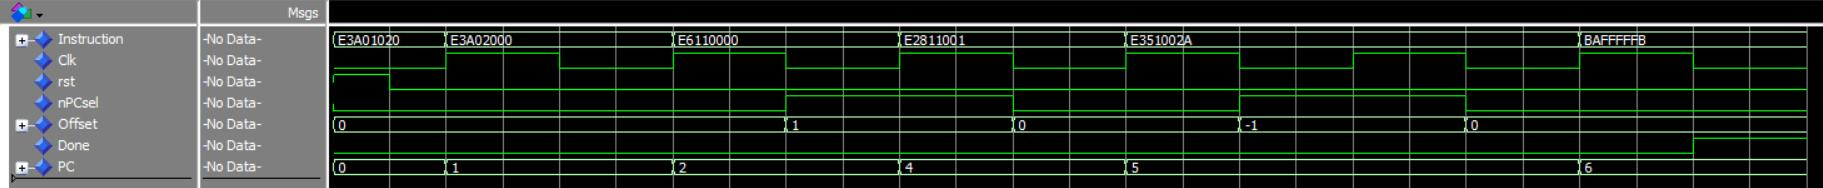
\includegraphics[width=1\textwidth]{picture/IMUres.jpg}
    \caption{Simulation of Instruction Management Unit}     
    \label{fig:IMUres}
\end{figure}

It can be seen clearly that \texttt{PC} change itself as we expected.
